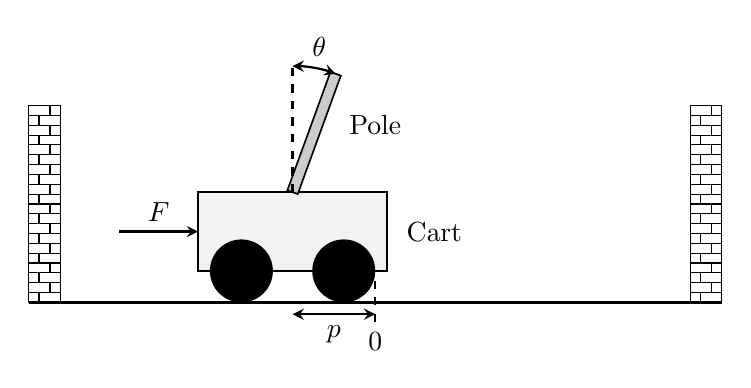
\begin{tikzpicture}[>=stealth]

% Ground and walls
\draw[thick] (-4.4, 0) -- (4.4, 0);
\draw (-4.4, 0) rectangle (-4, 2.5);
\draw (4, 0) rectangle (4.4, 2.5);

\foreach \x in {0,0.125,...,2.5} {
	\draw (-4.4, \x) -- (-4, \x);
	\draw (4, \x) -- (4.4, \x);
}

\foreach \x in {0,0.25,...,2.25} {
	\draw (-4.27, \x) -- (-4.27, \x+0.125);
	\draw (4.13, \x) -- (4.13, \x+0.125);
}

\foreach \x in {0.125,0.375,...,2.375} {
	\draw (-4.13, \x) -- (-4.13, \x+0.125);
	\draw (4.27, \x) -- (4.27, \x+0.125);
}

% Cart
\node at (0.75, 0.9) {Cart};
\filldraw[semithick, fill=black!5!white] (-2.25, 0.4) rectangle (0.15, 1.4);
\fill[black] (-0.4, 0.4) circle (0.4);
\fill[black] (-1.7, 0.4) circle (0.4);

\draw[thick, dashed] (0, -0.25) -- (0, 0.4);
\node at (0, -0.5) {$0$};

\node at (-0.525, -0.4) {$p$};
\draw[<->, thick] (-1.05, -0.15) -- (0, -0.15);

\node at (-2.75, 1.15) {$F$};
\draw[->, thick] (-3.25, 0.9) -- (-2.25, 0.9);

% Pole
\node at (0, 2.25) {Pole};
\filldraw[semithick, fill=black!20!white, rotate around={-20:(-1.05, 1.4)}] (-1.12, 1.4) rectangle (-0.98, 3);

\node at (-0.71, 3.25) {$\theta$};
\draw[thick, dashed] (-1.05, 1.4) -- (-1.05, 3);
\draw[<->, thick] (-1.05, 3) arc (90:70:1.6);

\end{tikzpicture}